% Provenance (never printed): see sources/outline_sources.md (Year 3:
% speciation and saturation indices; carbonate equilibria applied to rocks;
% weathering kinetics; hydrothermal fluids). Brief: sources/book5/BRIEFS.md,
% ch. 15. Curves from figdata/bachelor-3/carbonate_system.py,
% activity_diagram.py, weathering_rates.py. Exercise and problem values in the
% Book 5 scratch calculator calc/ch15.py. The spring below the Varden
% limestone, its analysis and the granite stream are invented.
\chapter{التفاعل بين الماء والصخر}\label{ch:b3:water-rock-interaction}

ينبوع عند سفح منحدر من الحجر الجيري يترك قشرة بيضاء على كل
غصن وحجر يلامسه؛ وجدول يصرّف الغرانيت يحمل السيليكا والصوديوم
والقليل من البوتاسيوم، ولا يترك أي قشرة على الإطلاق. ويكمن الفرق في
كيمياء الماء، والكيمياء سجلّ للصخر الذي عبره الماء
هو: كم من ثاني أكسيد الكربون حمل، وكم من الوقت بقي، وأيّ
المعادن أذاب وأيّها بنى. يقرأ هذا الفصل ذلك السجلّ بأدوات
كيمياء المحاليل، من تحليل الماء إلى معدّلات
ذوبان المعادن وآثار النظائر للموائع الحارّة في القشرة.

\begin{recall}
النشاط، ومعامل النشاط، والقوة الأيونية، وتوزيع الأنواع، وجداء الذوبان
القلوية، وحالة التشبّع $\Omega$، وقانون هنري، وقوانين المعدّل،
وقانون أرينيوس، والحالة الانتقالية، وقيمة $\delta$ موجودة في
المجلدات الجامعية لكتب الكيمياء. والتجوية الكيميائية، والتحلّل المائي
للسيليكات، ومعادن الطين والكاولينيت، موجودة في مجلد السنة الأولى، في فصله
عن التجوية والطين؛ وحدّ الانحلال وعمق التعويض
الكربوني في فصله عن رواسب الكربونات والسيليس والتبخّريات. والمائع الحراري
موجود في مجلد السنة الثانية، في فصله عن ترسّبات الخامات،
والمنظّم الحراري للتجوية السيليكاتية في فصله عن المناخ عبر
الزمن الجيولوجي؛ والدوران الحراري المائي موجود في كتب المدرسة.
\end{recall}

\section{تحليل ماء طبيعي}\label{sec:b3:water-rock-interaction:analysis}

يسرد تحليل الماء الأيونات الرئيسة بالمليغرام في اللتر: الكالسيوم،
والمغنيسيوم والصوديوم والبوتاسيوم؛ والبيكربونات والكلوريد والكبريتات والنترات؛
والسيليكا المذابة بوصفها \ce{SiO2}؛ والحموضة ودرجة الحرارة المقاستان عند
المنبع، لأنهما يتغيّران بمجرّد خروج العيّنة منه. ويُقسم على الكتلة
المولية فنحصل على المليمولات في اللتر، ويُضرب في الشحنة فنحصل على
المليمكافئات. والماء المخفّف متعادل كهربائيًا، فمجموع
الكاتيونات يساوي مجموع الأنيونات.

\begin{method}[التحقّق من تحليل ماء]\label{met:b3:water-rock-interaction:analysis}
\begin{enumerate}
\item حوّل كل تركيز إلى \unit{mmol/L} وإلى \unit{meq/L}؛
\item اجمع الكاتيونات والأنيونات بوحدة \unit{meq/L}؛
\item احسب خطأ توازن الشحنة $100\,(\sum\text{كاتيون} -
  \sum\text{أنيون})/(\sum\text{كاتيون} + \sum\text{أنيون})$، بالنسبة المئوية؛
\item اقبل التحليل إذا كان الخطأ ضمن 1 أو \qty{2}{\percent} لماء
  تتراوح أملاحه بين 250 و\qty{1000}{mg/L}، ويُسمح بخطأ أكبر قليلًا لماء أشدّ تخفيفًا؛
  وإلا فابحث عن أيون ناقص أو خطأ تحليلي.
\end{enumerate}
\end{method}
% ledger: hem85:charge-balance

ويساوي نشاط الأيون مولاليّته مضروبةً في معامل نشاطه
$\gamma$. وفي المياه الطبيعية يُحسب $\gamma$ من القوة الأيونية $I =
\tfrac12\sum m_i z_i^2$ باستخدام معادلة ديباي--هوكل الموسّعة
\[
-\log\gamma_i = \frac{A z_i^2\sqrt I}{1 + B a_i\sqrt I},
\]
حيث $A = 0.5085$ و$B = 0.3281$ للماء عند \qty{25}{\celsius}،
وحجم الأيون $a_i$ بالأنغستروم: 9 لأيون \ce{H+}، 8 لأيون \ce{Mg^2+}،
6 لأيون \ce{Ca^2+}، 5 لأيون \ce{CO3^2-}، 4 لأيونات \ce{Na+}، \ce{HCO3-} و\ce{SO4^2-}،
3 لأيونات \ce{K+}، \ce{Cl-}، \ce{OH-} و\ce{NO3-}. وتصلح المعادلة حتى
نحو \qty{0.1}{mol/L} من الأملاح أحادية التكافؤ، وهذا يشمل الأنهار ومعظم
المياه الجوفية، لكنها لا تشمل مياه البحر ولا المحاليل الملحية. وتغيّر الحرارة قيمة $A$ فقط من
0.4883 عند \qty{0}{\celsius} إلى 0.5425 عند \qty{60}{\celsius}، لذا تصلح القيم عند
\qty{25}{\celsius} للمياه الباردة أيضًا.
% ledger: hem85:debye-huckel

يتوزّع الكربون غير العضوي في الماء بين ثاني أكسيد الكربون المذاب
(ويُكتب \ce{CO2} لمجموع \ce{CO2} و\ce{H2CO3})، والبيكربونات
والكربونات، وترتبط فيما بينها بالعلاقات الآتية
\[
K_1 = \frac{a_{\ce{HCO3-}}\,a_{\ce{H+}}}{a_{\ce{CO2}}}, \qquad
K_2 = \frac{a_{\ce{CO3^2-}}\,a_{\ce{H+}}}{a_{\ce{HCO3-}}}, \qquad
K_H = \frac{a_{\ce{CO2}}}{P_{\ce{CO2}}},
\]
حيث $\log K_1 = -6.35$، و$\log K_2 = -10.33$، و$\log K_H = -1.47$ عند
\qty{25}{\celsius}، و$-6.46$ و$-10.49$ و$-1.27$ عند \qty{10}{\celsius}
($P$ بالضغط الجوي). وبين \mbox{\textdir TLT pH 6.4} و10.3 تغلب البيكربونات، وفي
معظم المياه الطبيعية تكون القلوية فيها بيكربونات تقريبًا كلها. وقيمة pH المقاسة
والبيكربونات المقاسة تعطي النوعين الآخرين، والضغط الجزئي لثاني أكسيد الكربون الذي
يكون الماء في حالة توازن معه.
% ledger: phreeqc:carbonate

\section{التشبّع}\label{sec:b3:water-rock-interaction:saturation}

\begin{definition}[مؤشّر التشبّع]\label{def:b3:water-rock-interaction:si}
\emph{مؤشّر التشبّع (للمعدن)}\index{مؤشّر التشبّع (للمعدن)}
في الماء هو $\mathrm{SI} = \log(\mathrm{IAP}/K)$، حيث IAP هو
ناتج نشاط الأيونات في الماء، مكتوبًا على غرار جداء
الذوبان للمعدن $K$: $\mathrm{SI} = \log\Omega$.
\end{definition}

الماء الذي فيه $\mathrm{SI} < 0$ يستطيع أن يُذيب المعدن، والذي فيه
$\mathrm{SI} > 0$ يستطيع أن يرسّبه، و$\mathrm{SI} = 0$ يمثّل حالة التوازن.
ولأنّ الطاقة الحرّة لتفاعل الذوبان هي $\Delta_r G = RT\ln\Omega
= 2.303\,RT\,\mathrm{SI}$، ويُعدّ مؤشّر التشبّع كذلك مقياسًا
للقوة الدافعة بوحدات $2.303\,RT$، أي نحو \qty{5.7}{kJ/mol} عند
\qty{25}{\celsius}. وبالنسبة إلى الكالسيت $\mathrm{IAP} = a_{\ce{Ca^2+}}
a_{\ce{CO3^2-}}$ و$\log K = -8.45$ عند \qty{25}{\celsius}، و$-8.35$ عند
\qty{10}{\celsius}: الكالسيت أشدّ ذوبانًا في الماء البارد. وبالنسبة إلى الجبس، $\mathrm{SI} = \log(a_{\ce{Ca^2+}}a_{\ce{SO4^2-}}) + 4.55$؛
وبالنسبة إلى الكوارتز، الذي يعطي ذوبانه \ce{H4SiO4} المتعادل، $\mathrm{SI} = \log
a_{\ce{H4SiO4}} + 3.98$، وبالنسبة إلى السيليكا غير المتبلورة يكون الثابت 2.71
بدلًا من 3.98. وتحمل المؤشّرات المقاسة عدم يقين لا يقلّ عن $\pm0.1$،
ويُعدّ الماء الذي يقع ضمن $\pm0.3$ من الصفر قريبًا من التوازن.
% ledger: phreeqc:carbonate, phreeqc:silicates, hem85:si

\section{توازنات الكربونات في الصخور}\label{sec:b3:water-rock-interaction:carbonate}

يذوب الكالسيت في الماء المشحون بثاني أكسيد الكربون وفق
\[
\ce{CaCO3 + CO2 + H2O <=> Ca^2+ + 2 HCO3-},
\qquad K = \frac{a_{\ce{Ca^2+}}\,a_{\ce{HCO3-}}^2}{P_{\ce{CO2}}}
= \frac{K_{\mathrm{cal}}K_1K_H}{K_2},
\]
مع $\log K = -5.94$ عند \qty{25}{\celsius} و$-5.59$ عند \qty{10}{\celsius}.
يتوقّف مقدار الذائب على مصدر ثاني أكسيد الكربون.

\begin{definition}[أنظمة الكربونات المفتوحة والمغلقة]\label{def:b3:water-rock-interaction:open-closed}
يذيب الماء الكالسيت في \emph{نظام الكربونات المفتوح}\index{نظام الكربونات المفتوح}
حين يبقى على تماسّ مع غاز
ذي $P_{\ce{CO2}}$ ثابت، يعوّض ثاني أكسيد الكربون المستهلك. ويفعل ذلك في
\emph{نظام الكربونات المغلق}\index{نظام الكربونات المغلق} حين يكون الماء قد
شُحن بثاني أكسيد الكربون أوّلًا، ثمّ عُزل عن الغاز، بحيث
يكون ثاني أكسيد الكربون الذي يحمله هو كلّ ما يستطيع استعماله.
\end{definition}

\begin{theorem}[ذوبانية الكالسيت في النظامين المفتوح والمغلق]\label{thm:b3:water-rock-interaction:calcite}
بالنسبة إلى ماءٍ من نوع بيكربونات الكالسيوم، حيث $m$ الملّالية للكالسيوم،
\[
\text{مفتوح:}\quad m = \left(\frac{K\,P_{\ce{CO2}}}{4\gamma_{\ce{Ca^2+}}
\gamma_{\ce{HCO3-}}^2}\right)^{1/3};
\qquad
\text{مغلق:}\quad 4\gamma_{\ce{Ca^2+}}\gamma_{\ce{HCO3-}}^2\,m^3 =
\frac{K_{\mathrm{cal}}K_1}{K_2}\,(C_0 - m),
\]
حيث $C_0 = K_H P_{\ce{CO2}}$ هو ثاني أكسيد الكربون الممتصّ قبل أن
ينغلق النظام.
\end{theorem}

\begin{proof}
بين الرقم الهيدروجيني 6.5 و8.5 تكون الكربونات و\ce{H+} و\ce{OH-} مهملةً مقارنةً
بالبيكربونات، ولذلك يكون ميزان الشحنة $2m = m_{\ce{HCO3-}}$. للنظام المفتوح: $K = \gamma
_{\ce{Ca^2+}}m\,\gamma_{\ce{HCO3-}}^2(2m)^2/P_{\ce{CO2}}$، فيُستخرج منه
الجذر التكعيبي. للنظام المغلق: كلُّ كالسيوم مُذاب يستهلك \ce{CO2} واحدًا، إذن $m_{\ce{CO2}}
= C_0 - m$ و$a_{\ce{Ca^2+}}a_{\ce{HCO3-}}^2/a_{\ce{CO2}} = K/K_H =
K_{\mathrm{cal}}K_1/K_2$ فتعطي المعادلة التكعيبية.
\end{proof}

في النظام المفتوح يتزايد الكالسيوم بقدر الجذر التكعيبي للضغط الجزئي $P_{\ce{CO2}}$؛ وفي
النظام المغلق يتقيّد الكالسيوم بالقيمة $C_0$، وثاني أكسيد الكربون المتبقّي عند
النهاية، ومن ثمّ $P_{\ce{CO2}}$ النهائي، أدنى كثيرًا مما في البداية. هواء
التربة يحمل من 10 إلى 100 ضعف ثاني أكسيد الكربون الموجود في الغلاف الجوي، يتولّد عن
الجذور وتحلّل المادة النباتية، وتُظهر المياه الجوفية عادةً
$P_{\ce{CO2}}$ بين $10^{-2.5}$ و$10^{-1}$ ضغط جوي. الماء الملامس
للكالسيت والهواء لا يحمل سوى نحو \qty{20}{mg/L} من الكالسيوم؛ والمطر الذي
يصل إلى الحجر الجيري عبر التربة، وما يزال مفتوحًا على غاز التربة، يستطيع أن
يحمل أكثر بأربع أو خمس مرّات. وتتشكّل الكارست بفعل ثاني أكسيد الكربون القادم من التربة.
% ledger: hem85:pco2, phreeqc:carbonate

ويتمثّل طريق العودة في خروج الغاز. والينبوع الخارج من الحجر الجيري يحمل
$P_{\ce{CO2}}$ الخاصّ بالتربة والصخر، من عشرة إلى مئة ضعف ما في
الهواء. وفي الهواء الطلق يفقد ثاني أكسيد الكربون، فتتحوّل البيكربونات إلى
كربونات، فيرتفع الرقم الهيدروجيني، ويزداد مؤشّر التشبّع بأكثر من وحدة واحدة،
كما تُبيّن اللوحة (ب) من الشكل أدناه بالنسبة إلى ينبوع
مسألة نهاية الأسبوع في هذا الفصل.
يترسّب الكالسيت على قاع الجدول وعلى الحزازيات والأغصان الصغيرة: التوفا من
الينابيع الباردة، والترافرتين من الينابيع الساخنة. والينابيع التي تعبر الصخر
بسرعة، خلال أيّام أو أسابيع، عبر القنوات، تصل عادةً إلى السطح
غير مشبعة؛ أمّا التي تترشّح ببطء عبره لشهور فتخرج قرب
حالة التشبّع.
% ledger: hem85:pco2, usgsyvo:travertine

\begin{omfigure}
\begin{tikzpicture}
\begin{groupplot}[group style={group size=2 by 1, horizontal sep=1.6cm},
  omrecord, width=0.47\linewidth, height=0.42\linewidth, title style={font=\small},
  tick label style={font=\scriptsize}, label style={font=\small},
  legend style={font=\scriptsize, legend cell align=left}]
\nextgroupplot[title={(أ) ذوبانية الكالسيت},
  xlabel={لوغاريتم الضغط الجزئي $\log P_{\ce{CO2}}$ \babelsublr{(atm)}}, ylabel={الكالسيوم المذاب \babelsublr{(\unit{mmol/L})}},
  xmin=-3.5, xmax=-1, ymin=0, ymax=5.5, clip=false,
  xtick={-3.5,-3,-2.5,-2,-1.5,-1}, xticklabels={$-3.5$,$-3$,$-2.5$,$-2$,$-1.5$,$-1$},
  legend style={at={(0.14,0.97)}, anchor=north west}]
\addplot[draw=none, fill=black!6, forget plot] coordinates {(-2.5,0) (-2.5,5.5) (-1,5.5) (-1,0)} -- cycle;
% computed in figdata/bachelor-3/carbonate_system.py
\addplot[omDef, thick] table[x=logp, y=ca_open10] {figdata/out/bachelor-3-carbonate_system-solubility.dat};
\addlegendentry{مفتوح، \qty{10}{\celsius}}
\addplot[red!70!black, thick] table[x=logp, y=ca_open25] {figdata/out/bachelor-3-carbonate_system-solubility.dat};
\addlegendentry{مفتوح، \qty{25}{\celsius}}
\addplot[omDef, thick, densely dashed] table[x=logp, y=ca_closed10] {figdata/out/bachelor-3-carbonate_system-solubility.dat};
\addlegendentry{مغلق، \qty{10}{\celsius}}
\addplot[red!70!black, thick, densely dashed] table[x=logp, y=ca_closed25] {figdata/out/bachelor-3-carbonate_system-solubility.dat};
\addlegendentry{مغلق، \qty{25}{\celsius}}
\draw[black, densely dotted] (axis cs:-3.37,0) -- (axis cs:-3.37,5.5);
\node[font=\scriptsize, anchor=south] at (axis cs:-3.37,5.5) {الهواء};
\node[font=\scriptsize, anchor=north] at (axis cs:-1.4,5.45) {المياه الجوفية};
\nextgroupplot[title={(ب) خروج الغاز من الينبوع},
  xlabel={لوغاريتم الضغط الجزئي $\log P_{\ce{CO2}}$ \babelsublr{(atm)}}, ylabel={مؤشّر التشبّع للكالسيت},
  xmin=-3.5, xmax=-1.5, ymin=-0.2, ymax=1.9, x dir=reverse, clip=false,
  xtick={-3.5,-3,-2.5,-2,-1.5}, xticklabels={$-3.5$,$-3$,$-2.5$,$-2$,$-1.5$}]
% computed in figdata/bachelor-3/carbonate_system.py
\addplot[omDef, thick] table[x=logp, y=si] {figdata/out/bachelor-3-carbonate_system-degassing.dat};
\addplot[black, densely dotted, domain=-3.5:-1.5, samples=2] {0};
\addplot[red!70!black, only marks, mark=*, mark size=1.6pt] table[x=logp, y=si] {figdata/out/bachelor-3-carbonate_system-ends.dat};
\node[font=\scriptsize, anchor=north west] at (axis cs:-1.84,-0.01) {المخرج};
\node[font=\scriptsize, anchor=north west] at (axis cs:-3.3,1.55) {الهواء};
\end{groupplot}
\end{tikzpicture}

\par\smallskip{\small (أ) الكالسيوم المذاب بالماء في حالة توازن مع
الكالسيت، بدلالة الضغط الجزئي لثاني أكسيد الكربون (بالنسبة إلى النظام المغلق،
الضغط الذي شُحن عنده الماء): النظام المفتوح بخط متّصل، والمغلق
بخط متقطّع؛ الماء البارد يذيب أكثر؛ والنطاق الرمادي هو مدى
المياه الجوفية. (ب) الينبوع الواقع أسفل حجر فاردن الجيري، عند \qty{10}{\celsius}،
يفقد ثاني أكسيد الكربون في طريقه إلى أسفل التلّ (يُقرأ من اليسار إلى اليمين، على محور معكوس)
قبل أن يتكوّن أيّ كالسيت: يثبت الكالسيوم والقلوية، ويرتفع الرقم الهيدروجيني
من 7.2 إلى 8.8، ويتغيّر مؤشّر تشبّعه من 0.04 إلى 1.6. وثوابت
التوازن مستمدّة من قاعدة بيانات عامة، ومعاملات النشاط بصيغة ديباي--هوكل
الموسّعة.}\label{fig:b3:water-rock-interaction:calcite}
\end{omfigure}
% ledger: phreeqc:carbonate, hem85:debye-huckel, hem85:pco2, data:co2-mlo

الكيمياء نفسها، مُطبَّقةً على مقياس المحيط، واردةٌ في المجلدات الجامعية من كتب الكيمياء؛ والعمقُ الذي تصبح عنده
مياهُ البحر غيرَ مشبعة بالكالسيت، وخطُّ الليزوكلاين، والعمقُ الذي
لا يتراكم تحته الكالسيت،
فكلُّها واردةٌ في مجلد السنة الأولى.

\begin{inthefield}[ينبوع يبني مصاطبه بنفسه]
\begin{minipage}[t]{0.52\linewidth}\vspace{0pt}
عند ينبوع باليت، أحد ينابيع ماموث الحارّة في هضبة يلوستون،
يصعد الماء الحراريّ عبر حجر جيري مدفون فيحمله مُذابًا
بعيدًا. وعلى السطح ينتشر الماء
فوق رواسبه الخاصّة، ويفقد ثاني أكسيد الكربون، فيترسّب كربونات الكالسيوم
على هيئة ترافرتين، أوّلًا على حافّة كلّ حوض حيث يكون الماء
أرقّ ما يكون. والجيولوجيّون الذين يمسحون هذه الينابيع يقيسون ترسّبًا يبلغ نحو
ثلاثة ملليمترات في اليوم، أي خمسة عشر ضعف معدّل التوفا في
الينابيع الباردة. والخطوط البرتقالية والبنّيّة
هي حصائر من الكائنات الدقيقة المحبّة للحرارة، تعيش في الجريان السطحي الدافئ.
\end{minipage}\hfill
\begin{minipage}[t]{0.44\linewidth}\vspace{0pt}
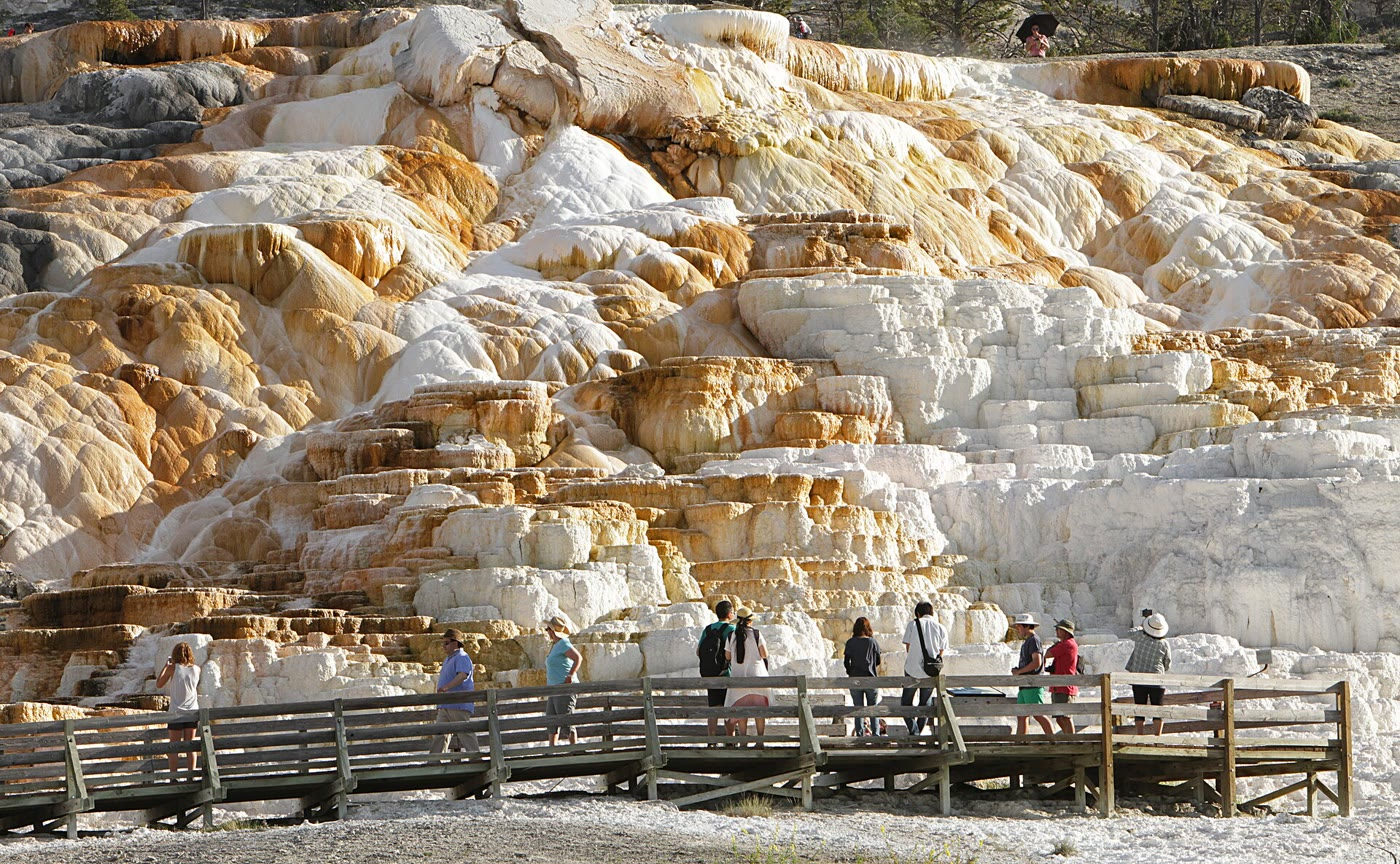
\includegraphics[width=\linewidth]{images/book5/b3-palette-spring-travertine.jpg}

{\scriptsize مصاطب الترافرتين في ينبوع باليت، ضمن ينابيع ماموث الحارّة، مع
ممشى خشبيّ وزوّار للمقارنة بالحجم. الصورة: NPS بتصوير \mbox{\textdir TLT Jim Peaco}، ملك عام.}
\end{minipage}
\end{inthefield}
% ledger: photo:b3-palette-spring, usgsyvo:travertine, nps:travertine-terraces

\section{حركيّة تجوية السيليكات}\label{sec:b3:water-rock-interaction:kinetics}

تذوب السيليكات أبطأ بكثير من الكالسيت، ونادرًا ما يبلغ الماء حالة التوازن معها:
ولذلك يلزم وصف ذوبانها بمعدّل.

\begin{definition}[قانون معدّل ذوبان المعادن]\label{def:b3:water-rock-interaction:rate-law}
\emph{قانون معدّل ذوبان المعادن}\index{قانون معدّل ذوبان المعادن} يُعطي
معدّل الذوبان لكلّ وحدة من مساحة سطح المعدن، بوحدة
\unit{mol.m^{-2}.s^{-1}}، على هيئة مجموع عبر الآليّات الحمضية والمتعادلة والقاعدية،
\[
r = \sum_j k_j\,e^{-\frac{E_j}{R}\left(\frac1T - \frac1{298.15}\right)}\,
a_{\ce{H+}}^{n_j}\,\bigl(1 - \Omega^{p_j}\bigr)^{q_j},
\]
مع ثوابت المعدّل $k_j$ عند \qty{25}{\celsius}، وطاقات التنشيط $E_j$،
ورتب التفاعل $n_j$ (سالبة للآليّة القاعدية)، والأُسّان
$p_j$، $q_j$، ويُؤخذان عادةً مساويين 1.
\end{definition}
% ledger: pk04:rate-law

\begin{proposition}[البعيد عن التوازن والقريب منه]\label{prop:b3:water-rock-interaction:affinity}
إذا كان $p = q = 1$، لا يتعلّق المعدّل بتشبّع الماء
حين $\Omega \ll 1$، وقرب التوازن يتناسب المعدّل طرديًّا مع
مؤشّر التشبّع: $r \approx -2.303\,r_\infty\,\mathrm{SI}$، حيث
$r_\infty$ هو المعدّل البعيد عن التوازن.
\end{proposition}

\begin{proof}
العامل هو $1 - \Omega = 1 - 10^{\mathrm{SI}}$. فعند $\mathrm{SI} \ll 0$ يؤول
إلى 1؛ أمّا عند $\mathrm{SI}$ قريبًا من الصفر، فإنّ $10^{\mathrm{SI}} \approx 1 +
2.303\,\mathrm{SI}$.
\end{proof}

تأتي ثوابت المعدّل من تجارب مخبريّة على مساحيق معدنيّة طازجة،
في مفاعلات جريانيّة تُبقى بعيدًا عن التوازن. يرسم الشكل أدناه
قانون المعدّل لأربعة معادن عند \qty{25}{\celsius}. كلّ منحنى هو على شكل V أو
U: تُسرّع البروتونات الذوبان في الماء الحمضي، والهيدروكسيد في الماء القاعدي، وفي
ما بينهما تشكّل الآليّة المتعادلة حدًّا أدنى. يذوب الأوليفين بنحو ثلاث
مراتب من القدر أسرع من الألبيت عند pH 5، ولهذا هو أوّل
السيليكات الشائعة التي تختفي من التربة. وطاقتا التنشيط للألبيت
والفورستيريت، من 65 إلى \qty{79}{kJ/mol}، تجعلان معدّليهما أسرع بأربع إلى خمس
مرّات عند \qty{25}{\celsius} منه عند \qty{10}{\celsius}.
% ledger: pk04:rates

معدّلات الحقل أدنى، بمراتب من القدر. وفي تجارب الأعمدة على
الجرانيت المطحون حديثًا، تراجع معدّل البلاجيوكلاز باطّراد خلال ست سنوات
إلى \qty{7.0e-14}{mol.m^{-2}.s^{-1}}؛ والجرانيت نفسه الذي تجوّى طبيعيًّا
وتحوّل جزئيًّا إلى الكاولينيت، ذاب بمعدّل \qty{2.1e-15}{mol.m^{-2}.s^{-1}}
تحت الظروف نفسها، وكلاهما ما زال أسرع بكثير من المعدّل
المقاس في مقطع التجوية نفسه. وعبر معادن وأعمار كثيرة، يتناقص
المعدّل مع الزمن $t$ الذي ظلّ المعدن يتجوّى خلاله، وفق $R =
\num{3.1e-13}\,t^{-0.61}$ (mol\,m$^{-2}$\,s$^{-1}$، $t$ بالسنوات). ويعود جزء
من التناقص إلى المعدن نفسه، إذ تذوب أكثر أسطحه تفاعلًا أوّلًا؛
أمّا الباقي فيعود إلى البيئة: ماءٌ بطيء، ومعدنٌ كثير لسائل قليل،
ومياه المسامّ القريبة من التوازن، حيث تجعل القضيّة أعلاه المعدّل
صغيرًا.
% ledger: whitebrantley03:rates

\begin{omfigure}
\begin{tikzpicture}
\begin{axis}[omrecord, width=0.74\linewidth, height=0.46\linewidth,
  xlabel={الرقم الهيدروجيني \babelsublr{(pH)}}, ylabel={المعدّل $\log r$ \babelsublr{(\unit{mol.m^{-2}.s^{-1}})}},
  xmin=0, xmax=14, ymin=-14.5, ymax=-6, clip=false,
  xtick={0,2,4,6,8,10,12,14}, ytick={-14,-12,-10,-8,-6},
  yticklabels={$-14$,$-12$,$-10$,$-8$,$-6$},
  tick label style={font=\scriptsize}, label style={font=\small},
  legend style={font=\scriptsize, legend cell align=left, at={(1.03,0.5)}, anchor=west}]
% computed in figdata/bachelor-3/weathering_rates.py
\addplot[green!45!black, thick] table[x=ph, y=forsterite] {figdata/out/bachelor-3-weathering_rates-curves.dat};
\addlegendentry{فورستيريت}
\addplot[omDef, thick] table[x=ph, y=albite] {figdata/out/bachelor-3-weathering_rates-curves.dat};
\addlegendentry{ألبيت}
\addplot[red!70!black, thick, densely dashed] table[x=ph, y=kfeldspar] {figdata/out/bachelor-3-weathering_rates-curves.dat};
\addlegendentry{فلسبار البوتاسيوم}
\addplot[black, thick, densely dotted] table[x=ph, y=kaolinite] {figdata/out/bachelor-3-weathering_rates-curves.dat};
\addlegendentry{كاولينيت}
\end{axis}
\end{tikzpicture}

\par\smallskip{\small معدّلات الذوبان بعيدًا عن التوازن عند
\qty{25}{\celsius}، بدلالة pH، من تجميع منشور لمعاملات
المعدّل المخبريّة. فالفورستيريت، وهو الطرف الأوليفيني، لا يتضمّن له
التجميعُ آليّةً قاعدية؛ ويتوقّف منحناه عن الانخفاض عند الحدّ الأدنى المتعادل.}\label{fig:b3:water-rock-interaction:rates}
\end{omfigure}
% ledger: pk04:rates

\begin{definition}[أنظمة التجوية]\label{def:b3:water-rock-interaction:regimes}
تكون التجوية الكيميائية في مشهد طبيعي في حالة
\emph{النظام المحدود بالإمداد}\index{النظام المحدود بالإمداد} عندما تتقيّد بالمعدّل الذي تجلب به التعريةُ
معادنَ طازجة إلى الجبهة التجويّة، وتكون في
\emph{النظام المحدود بالتجوية}\index{النظام المحدود بالتجوية} عندما تكون المعادن الطازجة وفيرة
ويحدّ من التجوية معدّلُ التفاعلات.
\end{definition}

يُظهر تجميعٌ لأحواض صغيرة النظامين معًا. فحيث تكون التعرية بطيئة، تحت تربة سميكة مغسولة
على تضاريس هادئة، يتبع دفقُ التجوية
معدّلَ التعرية: فكلّ صخرة طازجة تصل تُغسل كليًّا، ولا يغيّر المناخُ الأدفأ أو
الأرطب إلا تغييرًا يسيرًا. وحيث تكون التعرية سريعة، في الجبال الشديدة الانحدار، يزداد
الدفقُ مع الجريان السطحي، بوصفه الجذرَ التربيعي لمعدّل التعرية،
ومع درجة الحرارة، بطاقة تنشيط ظاهرية قدرها $74 \pm
\qty{29}{kJ/mol}$. ولا تستطيع التجوية السيليكاتية إلا في النظام الثاني أن تعمل
منظِّمًا لحرارة المناخ الوارد في مجلد السنة الثانية.
% ledger: west05:regimes

يُحدَّد المعدن الثانوي الذي تكوّنه مياهُ التجوية
بقراءة مخطط آخر.

\begin{definition}[مخطط النشاط]\label{def:b3:water-rock-interaction:activity-diagram}
\emph{مخطط النشاط}\index{مخطط النشاط} يقسّم مستوى نسب النشاط
لماءٍ ما، مثل
$\log(a_{\ce{K+}}/a_{\ce{H+}})$ مقابل $\log a_{\ce{H4SiO4}}$، إلى
الحقول التي يكون فيها كلُّ معدن من النظام الكيميائي هو المستقرّ.
\end{definition}

\begin{proposition}[حدود مخطط النشاط]\label{prop:b3:water-rock-interaction:boundaries}
في النظام \ce{K2O}--\ce{Al2O3}--\ce{SiO2}--\ce{H2O}، مع حفظ الألومنيوم في الأطوار الصلبة
والماء بنشاط الوحدة، لمعدنٍ ذي $k$ من ذرّات البوتاسيوم، و$a$ من ذرّات الألومنيوم،
و$s$ من ذرّات السيليكون في الصيغة الواحدة، وثابت الذوبان $K$ (إلى
\ce{K+}، \ce{Al^3+}، و\ce{H4SiO4})، يُحدَّد
\[
\log\frac{a_{\ce{Al^3+}}}{a_{\ce{H+}}^3} = \frac{\log K - kX - sY}{a},
\qquad X = \log\frac{a_{\ce{K+}}}{a_{\ce{H+}}},\quad Y = \log a_{\ce{H4SiO4}}.
\]
يعطي المعدنُ المستقرّ أدنى نشاط للألومنيوم، والحدّ الفاصل
بين معدنين خطٌّ مستقيم في $(Y, X)$.
\end{proposition}

\begin{proof}
يستهلك الذوبانُ $h = k + 3a$ بروتونًا، بحسب توازن الشحنة، ومنه $a\log
a_{\ce{Al^3+}} = \log K + h\log a_{\ce{H+}} - k\log a_{\ce{K+}} - s\log
a_{\ce{H4SiO4}}$؛ بقسمة على $a$ ونقل $3\log a_{\ce{H+}}$ إلى الطرف الأيسر
فنحصل على العبارة. والماءُ المتوازن مع معدن واحد يكون
غيرَ مشبع بأيّ معدن يتطلّب ألومنيومًا أكثر، وفوقَ التشبّع
بأيّ معدن يتطلّب ألومنيومًا أقلّ، فيكون الأقلّ ذوبانًا هو
المستقرّ. وبمساواة عبارتين من هذا النوع، وهما خطّيّتان في $X$ و$Y$، نحصل على خطّ مستقيم.
\end{proof}

مع الثوابت عند \qty{25}{\celsius}، يتحوّل الجيبسيت إلى الكاولينيت عند
$\log a_{\ce{H4SiO4}} = -4.39$ (\qty{2.4}{mg/L} من السيليكا)، ويتحوّل الكاولينيت إلى
الموسكوفيت عند $\log(a_{\ce{K+}}/a_{\ce{H+}}) = 1.55$، ويكون الفلسبار البوتاسي مستقرًّا
إلا في المياه الغنية بالبوتاسيوم والسيليكا. ويمثّل المخطط
تسلسلَ التجوية الوارد في مجلد السنة الأولى بلغة الأرقام: مياهٌ مخفّفة تجرف
البوتاسيوم والسيليكا بعيدًا فتُجرّد الفلسبارَ حتّى الجيبسيت؛ ومياهٌ تُبقي
على مزيد من السيليكا فتُكوّن الكاولينيت؛ ومياهٌ تُبقي على مزيد من البوتاسيوم، كما في الأعماق،
فتُكوّن الميكا.
% ledger: phreeqc:silicates

\begin{omfigure}
\begin{tikzpicture}
\begin{axis}[omrecord, width=0.66\linewidth, height=0.5\linewidth,
  xlabel={$\log a_{\ce{H4SiO4}}$}, ylabel={$\log(a_{\ce{K+}}/a_{\ce{H+}})$},
  xmin=-6, xmax=-2, ymin=0, ymax=10, clip=false,
  xtick={-6,-5,-4,-3,-2}, xticklabels={$-6$,$-5$,$-4$,$-3$,$-2$},
  tick label style={font=\scriptsize}, label style={font=\small}]
% computed in figdata/bachelor-3/activity_diagram.py
\addplot[black, thick, unbounded coords=jump] table[x=y, y=x] {figdata/out/bachelor-3-activity_diagram-lines.dat};
\addplot[omDef, densely dashed] table[x=y, y=x] {figdata/out/bachelor-3-activity_diagram-quartz.dat};
\addplot[omDef, densely dotted] table[x=y, y=x] {figdata/out/bachelor-3-activity_diagram-amorph.dat};
\addplot[red!70!black, only marks, mark=*, mark size=1.8pt] table[x=y, y=x] {figdata/out/bachelor-3-activity_diagram-samples.dat};
\node[font=\small] at (axis cs:-5.4,0.8) {الجيبسيت};
\node[font=\small] at (axis cs:-3.25,0.75) {الكاولينيت};
\node[font=\small] at (axis cs:-4.6,5.0) {الموسكوفيت};
\node[font=\small] at (axis cs:-3.3,9.3) {الفلسبار البوتاسي};
\node[font=\scriptsize, omDef, anchor=south] at (axis cs:-3.98,10) {الكوارتز};
\node[font=\scriptsize, omDef, anchor=south] at (axis cs:-2.71,10) {السيليكا غير المتبلورة};
\node[font=\scriptsize, red!70!black, anchor=west] at (axis cs:-4.58,0.38) {A};
\node[font=\scriptsize, red!70!black, anchor=west] at (axis cs:-3.80,1.29) {B};
\node[font=\scriptsize, red!70!black, anchor=west] at (axis cs:-3.48,4.08) {C};
\end{axis}
\end{tikzpicture}

\par\smallskip{\small حقول الاستقرار في النظام
\ce{K2O}--\ce{Al2O3}--\ce{SiO2}--\ce{H2O} عند \qty{25}{\celsius}، مع تشبّع الكوارتز
(بخط متقطّع) والسيليكا غير المتبلورة (بخط منقّط). ثلاث مياه مفترضة: A، جدول استوائيّ
مخفّف؛ B، جدول يجري على الجرانيت؛ C، المياه الجوفية العميقة في
الجرانيت.}\label{fig:b3:water-rock-interaction:activity}
\end{omfigure}
% ledger: phreeqc:silicates

\section{السوائل الحرمائية}\label{sec:b3:water-rock-interaction:hydrothermal}

تدور المياهُ الحارّة في القشرة قرب ظهرة أو كتلة متداخلة،
تتبادل الأكسجينَ مع الصخر الذي تعبره. وعند درجات الحرارة المرتفعة يكون
التجزّؤُ بين الصخر والماء صغيرًا، ويتحرّك كلاهما نحو
التوازن النظيري: فالماء الجوّي، وهو خفيف، يجعل الصخر أخفّ، والماء
أثقلَ. ويقيس مدى تحرّك الصخر كميّةَ الماء التي
مرّت به.

\begin{definition}[نسبة الماء إلى الصخر]\label{def:b3:water-rock-interaction:water-rock-ratio}
\emph{نسبة الماء إلى الصخر}\index{نسبة الماء إلى الصخر} $W/R$ لنظام حرمائيّ
هي كتلةُ الماء التي تبادلت مع كتلة من الصخر،
مقسومةً على تلك الكتلة من الصخر.
\end{definition}

\begin{proposition}[نسب الماء إلى الصخر من نظائر الأكسجين]\label{prop:b3:water-rock-interaction:wr}
ليكن صخرٌ قيمتُه الابتدائية $\delta_r^i$ يتبادل الأكسجين مع ماءٍ قيمتُه الابتدائية
$\delta_w^i$ حتّى يبلغ $\delta_r^f$، في توازن مع الماء
الذي التقى به آخرَ مرّة، $\Delta = \delta_r^f - \delta_w^f$، وليكن $c_r$ و$c_w$
تركيزَي الأكسجين في الصخر والماء. ففي نظام مغلق (دفعةٌ
واحدة من الماء) وفي نظام مفتوح (ماءٌ يمرّ مرّةً واحدة)،
\[
\frac WR\Big|_{\text{مغلق}} = \frac{c_r}{c_w}\,
\frac{\delta_r^f - \delta_r^i}{\delta_w^i - \delta_r^f + \Delta},
\qquad
\frac WR\Big|_{\text{مفتوح}} = \frac{c_r}{c_w}\,
\ln\!\left(\frac{\delta_r^f - \delta_r^i}{\delta_w^i - \delta_r^f + \Delta} + 1\right).
\]
\end{proposition}

\begin{proof}
المغلق: يُحفظ الأكسجين-18، $c_wW\delta_w^i + c_rR\delta_r^i = c_wW
\delta_w^f + c_rR\delta_r^f$، مع $\delta_w^f = \delta_r^f - \Delta$؛ نحلّ
من أجل $W/R$. المفتوح: كمية تفاضلية $\mathrm dW$ تدخل عند $\delta_w^i$ وتخرج في
حالة توازن مع الصخر، عند $\delta_r - \Delta$، إذن $c_rR\,\mathrm d\delta_r
= c_w(\delta_w^i - \delta_r + \Delta)\,\mathrm dW$. بفصل المتغيّرات،
$\int_{\delta_r^i}^{\delta_r^f}\mathrm d\delta_r/(\delta_w^i - \delta_r +
\Delta) = (c_w/c_r)\,W/R$، والتكامل هو $-\ln[(\delta_w^i - \delta_r^f
+ \Delta)/(\delta_w^i - \delta_r^i + \Delta)]$، وهو التعبير المطلوب.
\end{proof}

بالنسبة إلى الأكسجين، تقترب $c_r/c_w$ من 0.5. يحتاج النظام المفتوح دائمًا إلى ماء أقلّ من النظام المغلق
من الماء لتحقيق الانزياح نفسه، لأنّ كلّ كمية تخرج
أثقل ما يمكن. حول كثير من الاقتحامات يُظهر $\delta^{18}\mathrm O$ للصخر المحيط
نمطًا دائريًّا من القيم المنخفضة، تتراوح من نحو $+6$ إلى ما دون
0، ومركزه حيث مرّ أكبر قدر من الماء؛ وغالبًا ما تقع خامات السائل الحرمائي
داخل أدنى كفاف، وهو ما يجعل الخريطة أداةً
للاستكشاف.
% ledger: white13c9:water-rock

\begin{omfigure}
\begin{tikzpicture}[font=\small, >=Stealth]
\draw[thick, fill=black!6] (0,0) rectangle (4,2.2);
\node at (2,1.55) {\foreignlanguage{arabic}{الصخر، الكتلة $R$}};
\node at (2,0.95) {$\delta_r^i \to \delta_r^f$};
\node[font=\scriptsize] at (2,0.4) {\foreignlanguage{arabic}{التبادل عند درجة الحرارة $T$}};
\draw[->, thick, omDef] (-2.6,1.1) -- (-0.1,1.1);
\node[omDef, anchor=south, align=center, font=\scriptsize] at (-1.35,1.15) {\foreignlanguage{arabic}{الماء الداخل}\\\foreignlanguage{arabic}{$\delta_w^i$، $\mathrm dW$}};
\draw[->, thick, red!70!black] (4.1,1.1) -- (6.6,1.1);
\node[red!70!black, anchor=south, align=center, font=\scriptsize] at (5.35,1.15) {\foreignlanguage{arabic}{الماء الخارج}\\\foreignlanguage{arabic}{$\delta_r - \Delta$}};
\node[anchor=north, font=\scriptsize, align=center] at (2,-0.15) {النظام المفتوح: تمرّ كلّ كمية مرّةً واحدة وتخرج في\\توازن مع الصخر الذي التقت به آخرَ مرّة};
\end{tikzpicture}

\par\smallskip{\small نموذج الصندوق لنظام حرمائي. في النظام المغلق
تبقى دفعةٌ واحدة من الماء مع الصخر حتى يبلغا كلاهما حالة التوازن؛
في النظام المفتوح يمرّ الماء عبر الصخر، ويتحرّك الصخر نحو الماء قليلًا
مع كلّ كمية تمرّ.}\label{fig:b3:water-rock-interaction:box}
\end{omfigure}

\begin{definition}[نموذج مسار التفاعل]\label{def:b3:water-rock-interaction:reaction-path}
\emph{نموذج مسار التفاعل}\index{نموذج مسار التفاعل} يتتبّع
تركيبَ الماء والمعادنَ التي يكوّنها مع تقدّم التفاعل،
بإضافة كمّيات صغيرة من متفاعل (معدنٌ يذوب، أو غازٌ يخرج،
أو حرارةٌ تُسحب)، وإعادة حساب التوزيع النوعي ومؤشّرات التشبّع عند
كلّ خطوة، مع ترسيب أيّ معدن يبلغ حالة التشبّع.
\end{definition}

عند تطبيق \omterm{def:b3:water-rock-interaction:reaction-path}{نموذج مسار التفاعل} على ينبوع مسألة نهاية الأسبوع، مع إخراج الغاز خطوةً بخطوة،
يترسّب الكالسيت بمجرّد أن يتجاوز مؤشّره الصفر؛ وعند تطبيقه على
الغرانيت وماء المطر، يُنتج أوّلًا الجبسيت، ثم الكاولينيت، ثم
الميكا مع تجمّع السيليكا والبوتاسيوم في الماء، راسمًا مسارًا عبر
\omterm{def:b3:water-rock-interaction:activity-diagram}{مخطط النشاط}. تُنجز برامج التوزيع النوعي هذا باستعمال قواعد بيانات
ثوابت التوازن، مثل تلك المستعملة في هذا الفصل.
% ledger: phreeqc:silicates

\section{التمارين}

\begin{exercise}[$\star$]\label{exo:b3:water-rock-interaction:1}
يحتوي ماءٌ على (بوحدة \unit{mg/L}) \ce{Ca} 48، \ce{Mg} 9.7، \ce{Na} 23، \ce{K} 3.9،
\ce{HCO3} 183، \ce{Cl} 35.5 و\ce{SO4} 48. احسب الخطأ في موازنة
الشحنات. هل التحليل مقبول؟
\end{exercise}

\begin{exercise}[$\star$]\label{exo:b3:water-rock-interaction:2}
عند قوّة أيونية تساوي 0.0050، احسب معاملات النشاط
للأيونات \ce{Ca^2+}، \ce{HCO3-} و\ce{SO4^2-}.
\end{exercise}

\begin{exercise}[$\star$]\label{exo:b3:water-rock-interaction:3}
يحتوي ماءٌ يصرف من مارلٍ حاوٍ للجبس على \qty{3.0}{mmol/L} من الكالسيوم
و\qty{4.0}{mmol/L} من الكبريتات، عند قوّة أيونية تساوي 0.016. احسب
مؤشّر التشبّع للجبس. هل ما زال الماء قادرًا على إذابة الجبس؟
\end{exercise}

\begin{exercise}[$\star$]\label{exo:b3:water-rock-interaction:4}
تحتوي المياه الجوفية على \qty{12}{mg/L} من السيليكا، مُعبَّرًا عنها بصيغة \ce{SiO2}
وموجودةً بصيغة \ce{H4SiO4}. احسب مؤشّرَي التشبّع للكوارتز
وللسيليكا غير المتبلّورة عند \qty{25}{\celsius}.
\end{exercise}
% ledger: phreeqc:silicates

\begin{exercise}[$\star\star$]\label{exo:b3:water-rock-interaction:5}
بأخذ معاملات النشاط مساويةً للواحد، احسب كمية الكالسيوم المذابة بواسطة
نظامٍ مفتوح عند \mbox{\textdir TLT $P_{\ce{CO2}} = 10^{-2}$~atm}، عند \qty{25}{\celsius}
وعند \qty{10}{\celsius}، بالوحدتين \unit{mmol/L} و\unit{mg/L}.
\end{exercise}

\begin{exercise}[$\star\star$]\label{exo:b3:water-rock-interaction:6}
ماءٌ عند \qty{25}{\celsius} بدرجة حموضة \babelsublr{pH 7.60} و\qty{4.0}{mmol/L} من
البيكربونات. بمعاملات نشاط تساوي 1، احسب ثاني أكسيد الكربون
المذاب والكربونات، وضغطه الجزئي $P_{\ce{CO2}}$ ونسبة كلّ نوع في
الكربون غير العضوي المذاب.
\end{exercise}

\begin{exercise}[$\star\star$]\label{exo:b3:water-rock-interaction:7}
حبيبة الألبيت كرةٌ قطرها \qty{1}{mm} في ماء تربة ذي \babelsublr{pH 5} عند
\qty{25}{\celsius}، تذوب بالمعدّل المبيَّن في الشكل، $\log r = -12.09$.
بفرض أنّ الحجم المولي يساوي \qty{101.31}{cm^3/mol}، كم تبلغ سرعة
تناقص نصف قطرها، وكم يستغرق ذلك؟
\end{exercise}
% ledger: pk04:rates, phreeqc:silicates

\begin{exercise}[$\star\star$]\label{exo:b3:water-rock-interaction:8}
بأيّ عامل يتزايد معدّل الذوبان المحايد للألبيت ($E =
\qty{69.8}{kJ/mol}$) من \qty{5}{\celsius} إلى \qty{25}{\celsius}؟ وما
العامل المقابل لدفق التجوية مع $E = \qty{74}{kJ/mol}$؟
\end{exercise}
% ledger: pk04:rates, west05:regimes

\begin{exercise}[$\star\star$]\label{exo:b3:water-rock-interaction:9}
استنتج حدّ الكاولينيت--الموسكوفيت في \omterm{def:b3:water-rock-interaction:activity-diagram}{مخطط النشاط} انطلاقًا من
الثوابت $\log K = 7.435$ (للكاولينيت، \mbox{\textdir TLT 2 Al}، \mbox{\textdir TLT 2 Si}) و$12.703$ (للموسكوفيت، \mbox{\textdir TLT 1 K}،
\mbox{\textdir TLT 3 Al}، \mbox{\textdir TLT 3 Si}). ماءٌ عند \qty{25}{\celsius} يحتوي على \qty{2.0}{mg/L} من
البوتاسيوم، و\qty{15}{mg/L} من السيليكا، و\babelsublr{pH 7.0}: أيّ معدن يكوّنه؟
\end{exercise}
% ledger: phreeqc:silicates

\begin{exercise}[$\star\star\star$]\label{exo:b3:water-rock-interaction:10}
قرب تداخلٍ ناريّ، يُوجد غرانوديوريت بقيمة $\delta^{18}\mathrm O = +6$
عند $-2$ (\unit{\permil}). كان لماء الأمطار القيمة $-13$، وعند
درجة حرارة التبادل كانت الصخرة أثقل من
الماء بمقدار \qty{2}{\permil}. مع $c_r/c_w = 0.5$، احسب \omterm{def:b3:water-rock-interaction:water-rock-ratio}{نسبة الماء إلى الصخر}
لنظامٍ مغلق ولنظامٍ مفتوح، وفسّر سبب اختلافهما.
\end{exercise}
% ledger: white13c9:water-rock

\begin{exercise}[$\star\star\star$]\label{exo:b3:water-rock-interaction:11}
مطرٌ محمّل بغاز التربة بضغط جزئي \mbox{\textdir TLT $P_{\ce{CO2}} = 10^{-1.5}$~atm} عند
\qty{10}{\celsius} يصل إلى حجر جيري. بمعاملات نشاط تساوي 1،
احسب الكالسيوم الذي يذوبه إذا بقي مفتوحًا على غاز التربة، وإذا
عُزل عنه أوّلًا. ما الكسر من ثاني أكسيد الكربون المتبقّي في
الحالة المغلقة، وما قيمة $P_{\ce{CO2}}$ النهائية له؟
\end{exercise}

\begin{exercise}[$\star\star\star$]\label{exo:b3:water-rock-interaction:12}
باستخدام القضية المتعلّقة بالمعدّلات قرب الاتزان، ما الكسر من معدّله
بعيدًا عن الاتزان الذي يذوب عنده معدنٌ عند $\mathrm{SI} =
-2$، و$-1$، و$-0.1$؟ معدّل مخبري قيس بعد \num{6} سنوات من التفاعل
يتبع قانون القوّة الوارد في الفصل: بأيّ عامل سيكون قد انخفض
بعد \num{10000} سنة؟ اجمع التأثيرين لتفسير سبب انخفاض معدّلات الحقل
إلى هذا الحدّ من الانخفاض.
\end{exercise}
% ledger: whitebrantley03:rates

\section{مسألة: الينبوع أسفل حجر فاردن الجيري}

\begin{problem}[{مسألة نهاية الأسبوع --- التحليل، وثاني أكسيد الكربون
والتشبّع لينبوع جيري مُختلَق، وجدول على الغرانيت}]
\label{pb:b3:water-rock-interaction:1}
ينبع الينبوع عند أسفل الحجر الجيري الجوراسي لتلال فاردن، عند
\qty{10}{\celsius} و pH يساوي 7.20. تحليله (بوحدة \unit{mg/L}): \ce{Ca}
112، \ce{Mg} 4.0، \ce{Na} 7.0، \ce{K} 1.2، \ce{HCO3} 340، \ce{Cl} 11،
\ce{SO4} 14، \ce{NO3} 9. عند \qty{10}{\celsius}: $\log K_{\mathrm{cal}} =
-8.35$، $\log K_1 = -6.46$، $\log K_2 = -10.49$، $\log K_H = -1.27$. استخدم
معادلة ديباي--هوكل الممدّدة الواردة في الفصل، وأهمل أزواج الأيونات، وخذ
الهواء عند $\log P_{\ce{CO2}} = -3.37$.

\medskip\noindent\textbf{الجزء الأول --- التحليل.}
\begin{enumerate}
\item حوّل التحليل إلى \unit{mmol/L}.
\item احسب خطأ توازن الشحنات. هل التحليل مقبول؟
\item احسب قوّة الأيونات.
\item احسب معاملات نشاط \ce{Ca^2+}، و\ce{HCO3-}،
  و\ce{CO3^2-}.
\item هل معادلة ديباي--هوكل الممدّدة صالحة هنا؟
\end{enumerate}

\medskip\noindent\textbf{الجزء الثاني --- ثاني أكسيد الكربون.}
\begin{enumerate}[resume]
\item احسب نشاط البيكربونات.
\item احسب نشاط ثاني أكسيد الكربون الذائب.
\item احسب $P_{\ce{CO2}}$ للينبوع. كم مرّة يفوق قيمته في الهواء،
  ومن أين يمكن أن يأتي ثاني أكسيد الكربون؟
\item احسب تركيز الكربونات ونصيب كل نوع في
  الكربون غير العضوي الذائب.
\item تحقّق من أنّ القلوية هي البيكربونات في معظمها تقريبًا.
\end{enumerate}

\medskip\noindent\textbf{الجزء الثالث --- التشبّع والترافرتين.}
\begin{enumerate}[resume]
\item احسب ناتج نشاط الأيونات ومؤشّر تشبّع الكالسيت
  عند المخرج.
\item هل الينبوع في توازن مع الكالسيت؟ وهل هو ينبوع قنوي أم
  بطيء ومنتشر؟
\item احسب الكالسيوم لنظام مفتوح في توازن مع الكالسيت عند
  $P_{\ce{CO2}}$ للينبوع، بمعاملات النشاط في السؤال 4،
  وقارن بالتحليل.
\item يتخلّص الماء من غازاته في الهواء قبل أن يتشكّل أيّ كالسيت. مع إبقاء
  نشاط البيكربونات ثابتًا، احسب الأس الهيدروجيني ومؤشّر تشبّعه.
\item قدّر الكالسيوم الذي يحتفظ به بعد أن يرسّب الكالسيت حتى يعود إلى
  التوازن مع الهواء (نظام مفتوح، ومعاملات النشاط عند قوّة الأيونات
  الجديدة $3m$)، وكتلة الكالسيت لكل لتر.
\item يتدفّق الينبوع بمعدّل \qty{2.0}{L/s} ويوزّع رسوبه على مساحة
  \qty{400}{m^2}. لو بقي كل ذلك الكالسيت هناك، بكثافة
  \qty{2.71}{g/cm^3}، فبأيّ سرعة سينمو الرسوب؟
\end{enumerate}

\medskip\noindent\textbf{الجزء الرابع --- جدول الغرانيت.} يجري جدول فوق
غرانيت فاردن، تحت تربة سميكة على منحدرات لطيفة، يحتوي (عند
\qty{25}{\celsius}) على \qty{1.2}{mg/L} من البوتاسيوم، و\qty{9.0}{mg/L} من
السيليكا، و pH يساوي 5.8.
\begin{enumerate}[resume]
\item احسب موقعه على \omterm{def:b3:water-rock-interaction:activity-diagram}{مخطط النشاط}.
\item أيّ معدن يكوّنه؟ احسب مؤشّر تشبّعه للكوارتز.
\item دون أيّ تركيز للسيليكا سيكوّن الجبسيت؟
\item عند أيّ أس هيدروجيني سيبلغ حدّ الكاولينيت--الموسكوفيت؟
\item احسب معدّل ذوبان فلدسبار البوتاسيوم في هذا الماء، بعيدًا عن
  الاتزان، من الوسائط $\log k = -10.06$، $n = 0.500$ (حمضي)؛
  $-12.41$ (متعادل)؛ $-21.20$، $n = -0.823$ (قاعدي).
\item هل تجوية هذه المنطقة المائية أرجح أن تكون محدودة بالإمداد أم
  محدودة بالتجوية؟ لماذا؟
\item مع طاقة تنشيط ظاهرية تساوي \qty{74}{kJ/mol}، بأيّ عامل سيتغيّر
  دفق محدود بالتجوية بين \qty{10}{\celsius}
  و\qty{25}{\celsius}؟
\item اذكر مؤشّر تشبّع الكالسيت لماء الينبوع عند
  مخرجه.
\end{enumerate}
\end{problem}
% ledger: phreeqc:carbonate, phreeqc:silicates, hem85:debye-huckel, hem85:charge-balance, hem85:si, hem85:pco2, pk04:rates, west05:regimes, data:co2-mlo
